\documentclass{astroedu-lab}

\begin{document}

\pagestyle{plain}

\begin{problem}{\huge Лабораторная работа 2.2.6\\\\Определение энергии активации\\\\по температурной зависимости\\\\вязкости жидкости\\\\Выполнил Жданов Елисей Б01-205}

\section{Цель работы:}

1) Измерение скорости падения шариков при разной температуре жидкости

2) Вычисление вязкости жидкости по закону Стокса и расчет энергии активации

\section{Оборудование:}

Стеклянный цилиндр с исследуемой жидкостью (глицерин)

Термостат

Секундомер

Горизонтальный компаратор

Микроскоп

Мелкие шарики (диаметром около 1 мм)

\section{Теоретическая справка}

Сила сопротивления для шарика в жидкости определена теоретически

\begin{equation}
	F = 6 \pi \eta r v
\end{equation}

Составив с использованием выражения уравнение вертикально движения шарика в жидкости и решив его, получим

\begin{equation}
	\eta = \frac{2}{9} g r^2 \frac{\rho - \rho_\text{ж}}{v_\text{уст}}
\end{equation}

\begin{equation}
	\tau = \frac{2}{9} \frac{r^2 \rho}{\eta}
\end{equation}

Также релаксационный путь будет равен

\begin{equation}
	S = v_\text{уст} \tau \left( \frac{t}{\tau} - 1 + e^{-t/\tau} \right)
\end{equation}

Плотность жидкости зависит от температуры, значения будем брать из графика

\begin{figure}[!h]
	\centering
	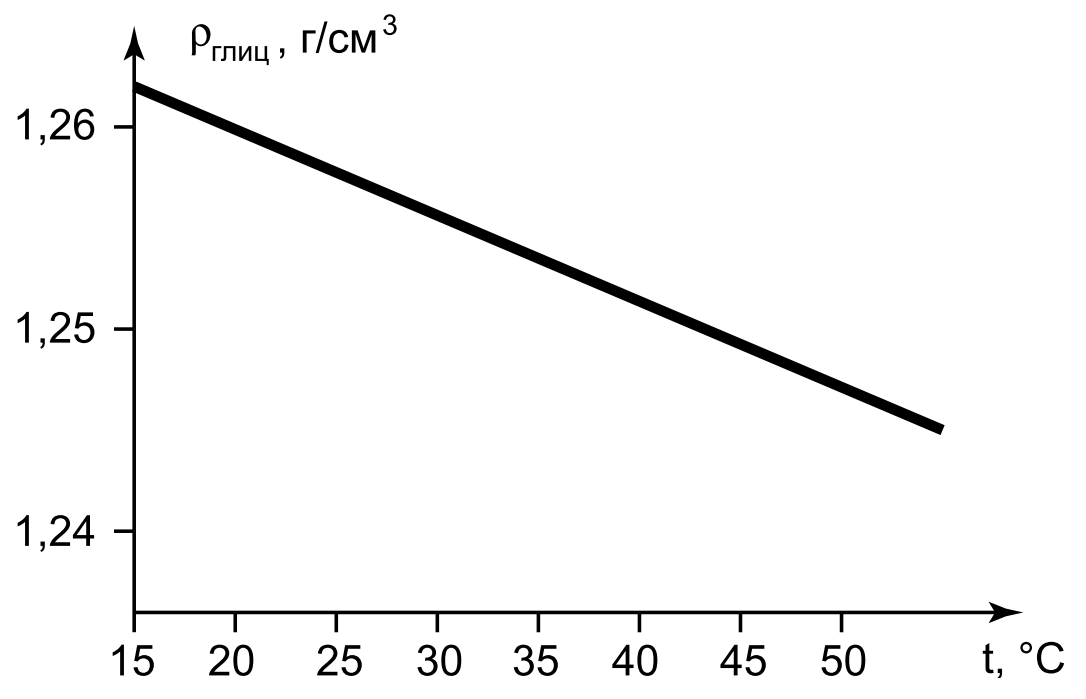
\includegraphics[width=0.75\textwidth]{плотность.png}
	\label{fig:boiler}
\end{figure}

Наконец, можно записать выражения для энергии активации

\begin{equation}
	W = k \frac{d(ln \eta)}{d(1/T)}
\end{equation}

Построим график в логарифмических координатах

\section{Экспериментальная установка}

\begin{figure}[!h]
	\centering
	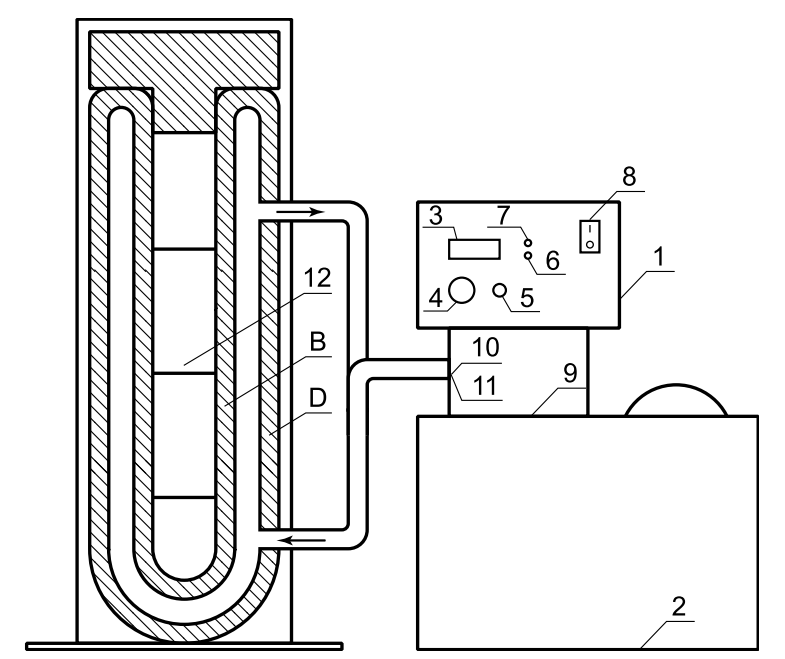
\includegraphics[width=0.9\textwidth]{установка.png}
	\label{fig:boiler}
\end{figure}

На стенках сосуда нанесены две метки на некотором расстоянии друг от друга. Верхняя метка располагается ниже уровня жидкости с таким расчетом, чтобы скорость шарика к моменту прохождения этой метки успевала установиться. Измеряя расстояние между метками с помощью линейки, а время падения с помощью секундомера, будем определять скорость шарика $v_\text{уст}$.

Радиусы шариков измеряются горизонтальным компаратором или микроскопом.

\section{Измерения, Обработка}

1-2) Радиус сосуда R = см

\begin{center}
\begin{tabular}{|c|c|c|c|}
\hline 
$\tau$, сек & $T$, К & d, мм & \\
\hline
188.0 & 188.0 & $(64.5 \pm 3.9)$ & 22\\
\hline
\end{tabular}
\end{center}


5) Найдем угловые коэффициенты прямых для каждой установки по МНК.

\[
	a = \frac{<x_i y_i> - < x > < y_i >}{< x_i^2> - < x_i >^2}
\]

\[
	b = < \nu_i > - a < N_i >
\]

Также рассчитаем их погрешности

\begin{equation}
	S_a^2 = \frac{< x_i^2>}{< x_i^2 > - < x_i >^2} \cdot \frac{<  b_i - b > ^2}{n - 2}
\end{equation}


\begin{center}
	\Large $q(T)$
\end{center}

%\begin{figure}[!h]
%	\centering
%	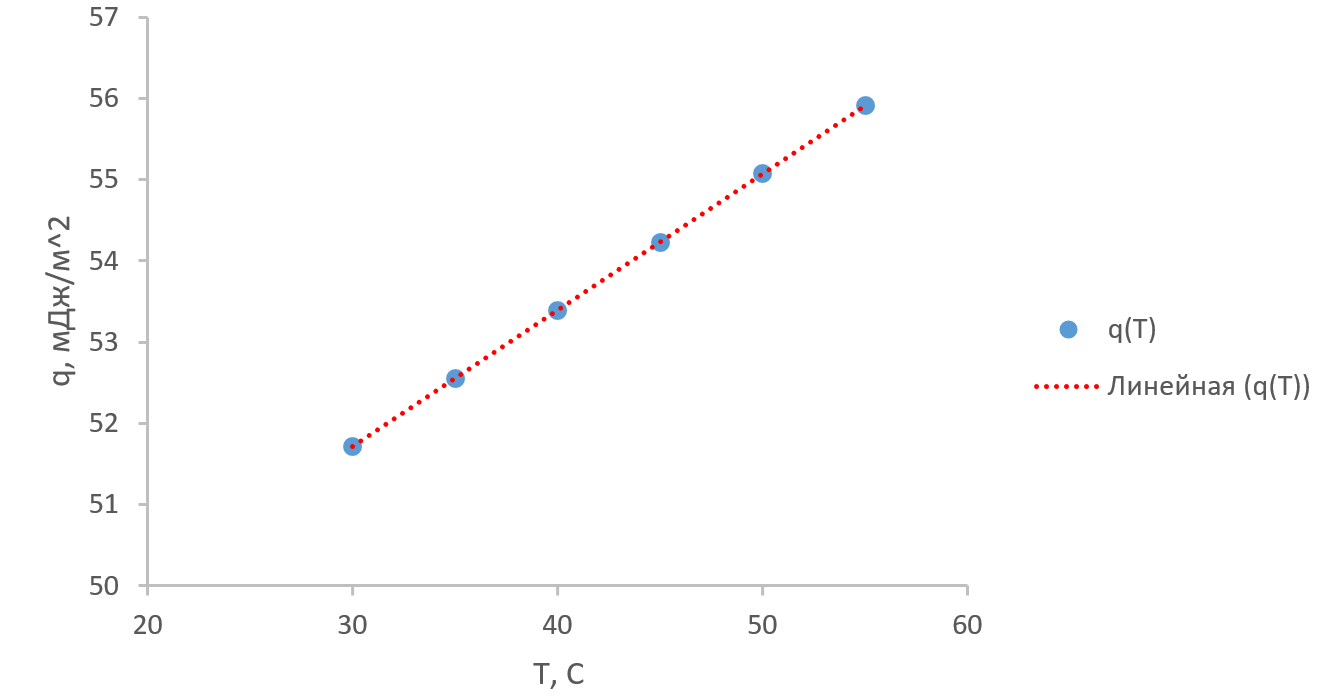
\includegraphics[width=1\textwidth]{2023-02-23_22-23-59.png}
%	\label{fig:boiler}
%\end{figure}

\section{Вывод}


\section{Ресурсы}

Расчет по МНК: метод-наименьших-квадратов.рф


\end{problem}
\end{document}